\documentclass[a4paper,twocolumn,10pt]{jsarticle}

\usepackage{geometry}
\geometry{top=20mm, bottom=24mm, left=23mm, right=23mm}

\makeatletter
  % maketitle
  \def\@maketitle{%
    \newpage
    \begin{center}%
     %和文題名
     {\Large \textbf{\@title} \par}%
     \vskip 9pt
     %和文著者
     {\large \lineskip .0em
     \begin{tabular}[t]{c}%
      \@author
     \end{tabular} \par}%
     %英文題名
     \vskip 1.5em
     {\Large \textbf{\etitle@etitle} \par}%
     \vskip 0.5em
     %英文著者
     {\large \lineskip .0em
     \begin{tabular}[t]{c}%
      \etitle@eauthor
     \end{tabular} \par}%
     \vskip 0.5em
    \end{center}%
    \par\vskip 1.5em
    \ifvoid\@abstractbox\else\centerline{\box\@abstractbox}\vskip1.5em\fi
    }
  % \title \author は既存のマクロを利用 \@title \author に値がセットされる.
  \newcommand{\etitle@etitle}{}
  \newcommand{\etitle@eauthor}{}
  \newcommand{\affiliation}[1]{\renewcommand{\etitle@affiliation}{#1}}
  \newcommand{\etitle}[1]{\renewcommand{\etitle@etitle}{#1}}
  \newcommand{\eauthor}[1]{\renewcommand{\etitle@eauthor}{#1}}
\makeatother

% !!!重要!!! ファイル先頭からこの行までの間は改変しないこと.

% 必要に応じて適宜パッケージを追加
% 例:特殊な数学記号を利用する→ \usepackage{amsmath} など
\usepackage[dvipdfmx]{graphicx}  % 図をインポートするパッケージ
\usepackage{url}       % URLを \url{} で括ると見やすくなる

% 和文題名
\title{宮下ゼミ卒業論文テンプレート2023}
% 和文著者
\author{京都女子大学 現代社会学部 現代社会学科 宮下ゼミ\\
20241000 西本 願子}
% 英文題名
\etitle{Manuscript Template for Graduation Thesis in Miyashita Lab 2023}
% 英文著者. 和文所属と同様です
\eauthor{Miyashita Lab., Faculty for the Contemporary Society, Kyoto Women's University\\
20241000 Nishimoto Ganko}

% 論文の概要
\begin{abstract}
本稿は京都女子大学現代社会学部宮下ゼミの学生向けに書かれた卒業論文のテンプレートであり,同時に卒論執筆の際の注意点などをまとめたものでもある.
主に \LaTeX の使い方に関する説明と,論文の内容に関して``するべきこと''と``するべきでないこと''をまとめている.
本稿自体も \LaTeX を利用して執筆されているので,卒論作成の参考になれば幸いである.
さて,本来この部分には卒業論文の概要(論文内容を簡潔にまとめたもの)を書く.
つまり研究の動機や背景,問題,解決手法,結論などを簡潔にまとめた文章を「概要」としてまとめる.
この概要を読めば論文内容がだいたい示されているようにすることが重要である(もともと「概要」とはそのようなものである).
文章量は特に定めないが,だいたい6〜8行程度にすればバランスがよいと思われる.
\end{abstract}

\begin{document}
% \begin{document} 直後に \maketitle コマンドを置く
\maketitle

\section{はじめに}

これは京都女子大学現代社会学部宮下ゼミ(以下,本ゼミという)の学生向けに書かれた卒業論文テンプレートである\footnote{本稿の最新版は\url{https://github.com/kensuke-m/graduationthesis-template}から入手できる.}.
本ゼミの学生はこの内容をよく理解し,すばらしい卒業論文を執筆してもらいたい.
また,このテンプレートに足りないところや誤りがあればいつでも指摘してほしい.

本ゼミの卒業論文はA4縦型2段組を採用している.
これは情報処理学会論文誌や研究報告と同様であり,卒業論文を執筆する学生にとっては演習Vで論文紹介をしたときに見慣れた体裁かと思われる.

本稿ではまず\LaTeX のスタイルファイルを用いた論文のフォーマットについて述べる.
論文フォーマットについて詳しくは\ref{sec:format}節で後述する指針を参照してほしい.
また,そこで説明されていることの外は標準的な \LaTeX のコマンドや他のスタイルファイルなどを利用して構わない.
本稿は卒業論文のテンプレートとして実際に \LaTeX を利用しているので,論文執筆時にはソースファイル({\tt main.tex})なども参考にされたい.

また,卒業論文を執筆する際に著者(これを読んでいるあなたである)がするべきこと,するべきでないこともまとめてある.
本稿の後半ではこれらについて指針を述べているので,卒論提出前はもとより執筆中にもぜひ継続的にチェックしていただきたい.

明確で簡潔に書かれた文書に勝るものはない.
第2次大戦中,イギリスのウィンストン・チャーチル首相は「我が国の外務省は長い報告書を書けばナチスに勝てると思っているようだ」としばしばこぼしたという\cite{newsweek2021}.
卒業論文(に限らず他人に読んでもらうことが目的の文書はすべてそうだが)は,できる限り短く,論旨が明確で,理解しやすいものを目指そう.

\section{卒業論文執筆の流れ}

卒業論文は以下のように執筆し,提出することが望ましい.

\subsection{準備}

必要なファイル一式は \url{https://github.com/kensuke-m/graduationthesis-template} から入手できる.
ここには以下のファイルが含まれる.
\begin{enumerate}
 \item \verb|graphs.png    |: 図で利用する画像ファイル
 \item \verb|ipsjunsrt.bst |: 参考文献リスト設定ファイル
 \item \verb|latexmkrc     |: \LaTeX の設定ファイル
 \item \verb|main.tex      |: 本稿のソースファイル
 \item \verb|README.md     |: 利用法の説明
 \item \verb|reference.bib |: 参考文献リスト
\end{enumerate}
これらのファイルの利用法は {\tt README.md} に書かれているので,まずはそれにしたがって卒論執筆の準備をしてほしい.
それが済んだら続きを読もう.

卒業論文はこのファイルのように文書処理システム \LaTeX を利用して作成し,PDF形式で提出する.
以前は \LaTeX を各自がPCにインストールして利用していたが,近年ではWWW上のアプリケーションとして利用するOverleaf\footnote{\url{https://ja.overleaf.com}}のようなシステムが普及しているので,それを使う.

\subsection{執筆}

本稿にしたがって卒業論文を執筆し,\LaTeX ソースファイルからPDFファイルを作成する.
前述した Overleaf では「リコンパイル」ボタンのクリックまたは Alt キーを押しながら Return キーを押下することでPDFファイルが作成され,WWWブラウザ内でプレビューできる.
その際エラーが発生すれば適宜修正し,プレビューできた場合は自分の意図通りの体裁になっているか,誤字や脱字などはないかなどをチェックする.
そして説明の足りないところを補ったり,図表を挿入してわかりやすくしたりなどの改善を繰り返しつつ,卒論を完成させる.

ある程度執筆が進んだらPDFファイルをダウンロードして紙に印刷してみることをお勧めする.
PCのディスプレイやタブレットなどの透過光で読む原稿と紙のように反射光で読む原稿では見え方が異なり,一方では気付かなかったことに他方で気付くことが多い.
特に完成した卒論を提出する直前には印刷したものを一度通して読んでみると良い.

自分ではこれ以上改善すべき箇所が見当たらないというところまで来たら,教員に提出してコメントをもらおう.
自分では気付かなかったことが必ずあるはずで,教員から何か所も指摘されるはずである.
提出までにこのような教員とのやりとりを数回繰り返し,卒論を改善してもらいたい.

\subsection{提出}

本ゼミでは卒業論文を提出する際に,ゼミ内での提出と教務課への提出の2つが要求される.
もちろん両方が必要である.

前者では,PDF形式のファイルを教員が指定した方法で然るべき場所へアップロードする.
具体的には,Microsoft Teams内のその年度の演習VIチャネルに「卒業論文」という課題が作成されるので,そこへPDFファイルをアップロードする.

後者は,印刷された原稿(左上をホチキス等で綴じること)を教務課窓口へ提出するのが通例である.
このとき,卒業論文題目用紙という紙を添付する必要があり,これは京女ポータル上で卒業論文のタイトルや指導教員名などを入力し,印刷したものに指導教員が押印する.
時期が来たら研究室の扉にシャチハタ印がぶら下げられるので各自で押印のこと\footnote{社会情勢の変化により提出方法が変更される可能性があるので京女ポータルのお知らせに注意すること.}.

どちらも2024年1月15日(月)17時が〆切であるが,少し余裕を持って提出できるよう計画すると良い\footnote{前年12月後半から受け付けてもらえるようである.}.

\section{卒業論文フォーマット}
\label{sec:format}

卒業論文は電子的な媒体で読む(例えばPCやタブレットの画面で閲覧する)のに適するよう作成し,PDF形式のファイルで提出する.
以下では卒業論文のフォーマットについて指針を述べるので,これにしたがって執筆すること.
\LaTeX を利用した文書作成について一般的な知識は \cite{okumura2020} を参考にされたい.

\subsection{卒業論文の構成}

卒業論文の \LaTeX ソースファイル({\tt main.tex})の構成は以下のようになる.

まず,ファイルの冒頭から\\
\verb|% !!!重要!!! ファイル先頭からこの行までの間は改変しないこと.|\\
と書かれた行までは改変せずそのまま利用する.

上記の行の直下には利用したい \LaTeX パッケージを列挙する.
図をインポートするパッケージである graphicx とURLを扱いやすくするための url パッケージを,例も兼ねてインクルードするように記述してあるので,他に必要なパッケージがあればそれらに倣うと良い.

その後,\verb|\title{表題(和文)}| と \verb|\author{著者(和文)}| および \verb|\etitle{表題(英文)}| と \verb|\eauthor{著者(英文)}| を例に倣って記述する.
表題は論文内容を端的に表すものとし,通常は体言止めとする.
表題は少し大きな字でセンタリングして出力される.
長い表題は適当な箇所に \verb|\\| を挿入して改行すると良い.
著者の所属は例のままとし,学生証番号と氏名を自分のものに変更する.
英文の表題は和文のものを翻訳し,英文の著者はローマ字で綴れば良い.

\verb|\begin{abstract}| から \verb|\end{abstract}| までの部分には論文の概要を書く.
ここには論文内容を簡潔にまとめた文章を記述し,ここを読めば論文内容がだいたい理解できるようにする.
文章の量については特に定めないが,少なくとも5,6行,多くても10行以内にするとバランスが良い.

そして \verb|\begin{document}| 以降 \verb|\end{document}| までが卒業論文の本文となる.
\verb|\begin{document}| 直下の \verb|\maketitle| は表題などをバランス良く出力するためのコマンドなので削除しないこと.

\subsection{本文}

本文は日本語または英語で記述し,日本語は常体で記述する\footnote{表題と著者のみ日本語と英語を併記する.}.
また,論文全体はA4判2段組で8ページ以下にまとめる.
プログラムのソースリストや詳細なアルゴリズムなどが長大になる場合は末尾に付録として追加し,これらは上記ページ数には含めないこととする.

\subsubsection{見出し}

本文は読みやすいようにいくつかの節\footnote{大抵の場合,「はじめに」で始まり,背景や先行研究,本論,考察などを述べ,「おわりに」で終わる.その後,謝辞と参考文献が続く.この原稿もそれに準じている.}や段落に分け,明瞭簡潔な記述を心がける.

節や小節の見出しには \verb|\section| や \verb|\subsection| を使用する.
この際,その直後に \verb|\label| を利用してラベルを付け,相互参照のために利用する\footnote{こうしておくと節の番号が変化しても自動的に追随するのでとても便利である.}.

\subsubsection{行送り}

改行位置や行間隔などは \LaTeX に任せるのが賢明である.
自動的に読みやすいレイアウトが手に入る.
そのため,本文中に \verb|\\| を挿入して強制的に改行したり \verb|\vspace| や \verb|\vskip| などで間隔を調整したりしないようにすること.

\subsubsection{フォント}

フォントサイズは \LaTeX が適切に設定するので,基本的に自分で設定する必要はない.
また,明朝体と{\bfseries ゴシック体}の利用も原則として \LaTeX に任せるのが良い.

\subsubsection{句読点}

句点には全角の「.」(ピリオド),読点には全角の「,」(コンマ)を用いる.
ただし,英文中や数式中でピリオドやコンマを使う場合は半角文字を利用する.
「。」や「、」は使わない.

\subsubsection{全角文字と半角文字}

全角文字と半角文字の両方が利用できる文字は以下のように使い分ける.

\begin{enumerate}
 \item 括弧は全角文字(「(」と「)」)を用いる.
       ただし,英文中では半角文字(「(」と「)」)を用いる.
 \item 英数字,空白,記号類は半角文字を用いる.
       ただし句読点は上述のように例外とする.
 \item カタカナは全角文字を用いる.
 \item 引用符は開きと閉じを区別する.
       開くときは \verb|``| を用い,閉じるときは \verb|''| を用いる.
\end{enumerate}

\subsubsection{箇条書き}

箇条書きは場合に応じて \verb|enumerate|,\verb|itemize|,\verb|descriprtion| を使い分けると良い.
箇条書きをあまり多用するのは好ましくないので,効果的に利用すること.

\subsubsection{脚注}

脚注は \verb|\footnote| コマンドを使う\footnote{これは脚注の例である.}.
参照したWWWサイトやWWW上の資料のURLは参考文献リストではなく脚注に記す.

脚注は本文を補う情報が必要なときに用いるが,括弧書きで文章に追記するか脚注とするかは統一的な基準があるわけではなく,各自で試行錯誤されたい.

\subsection{数式}

本文中の数式は \verb|$| と \verb|$| または \verb|\(| と \verb|\)| で囲んで記述する.
また,数式だけを別組みとするときは \verb|\[| と \verb|\]| で囲むか \verb|displaymath| や \verb|equation|,\verb|eqnarray| などの環境を用いる.
これらを利用すれば
\[
 S = \sum_{k=1}^{n}a_n
\]
のように,数式を見やすく配置できる.

\subsection{図}

1段の幅に収まる図は図\ref{fig:example1}の形式で指定する.
図の位置は \LaTeX に任せ,\verb|h| を使わずページの上端か下端に配置する.
また,図の下に見出しを \verb|\caption| で指定し,\verb|\label| でラベルを付して本文から \verb|\ref| コマンドで参照する.

\begin{figure}[tb]
\setbox0\vbox{
\hbox{\verb|\begin{figure}[tb]|}
\hbox{\quad \verb|<|図本体の指定\verb|>|}
\hbox{\verb|\caption{<|見出し\verb|>}|}
\hbox{\verb|\label{| $\ldots$ \verb|}|}
\hbox{\verb|\end{figure}|}
}
\centerline{\fbox{\box0}}
\caption{1段幅の図}
\label{fig:example1}
\end{figure}

図の内容として画像ファイルを指定する場合は graphicx パッケージの \verb|\includegraphics| コマンドを利用し,引数としてファイル名や大きさ(幅や高さ,拡大率など)を指定する(図\ref{fig:graphs}).
画像ファイルはできるだけ精細なものを利用すると見やすい出力が得られる.

\begin{figure}[tb]
 \begin{center}
  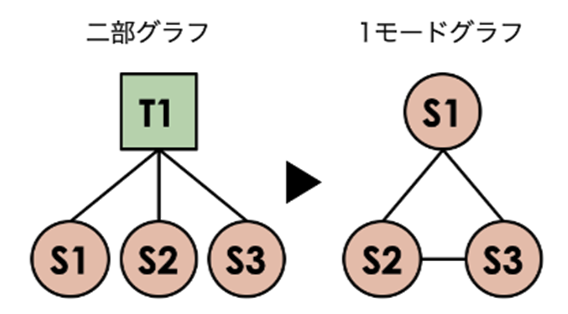
\includegraphics[width=0.9\linewidth]{graphs.png}
  \caption{2部グラフから1モードグラフへの変換}
  \label{fig:graphs}
 \end{center}
\end{figure}

また,2段の幅に跨る図は \verb|figure| 環境の変わりに \verb|figure*| 環境を利用すれば良い.

\subsection{表}

表は \verb|table| 環境を利用する\footnote{図と同様,2段の幅を使いたいときは \verb|table*| 環境を用いる.}.
表の例を表\ref{tab:competency} に示す.
表の上に見出しを \verb|\caption| で指定し,\verb|\label| で付けたラベルを \verb|\ref| コマンドで参照する.

表の罫線はなるべく少なくすると良い.
罫線はもっとも上のものを二重線とし,左右の端には縦の罫線を描かないようにするとすっきりする.

\begin{table}[tb]
 \begin{center}
  \caption{コンピテンシーディクショナリの項目数}
  \label{tab:competency}
  \begin{tabular}{c|ccc}
   \hline\hline
   名称 & タスク & スキル & 関連知識\\
   \hline
   項目数 & 639 & 491 & 8843\\
   分類 & 203 & 150 & 3308\\
   \hline
  \end{tabular}
 \end{center}
\end{table}

\subsection{謝辞}

研究を進めたり卒論を作成したりしたときにお世話になった人(指導教員,友人,知人,家族等)がいれば,謝辞に具体的に記して謝意を述べる.
謝辞は参考文献リストの直前に置き,\verb|acknowledgment| 環境を用いる.

この節の文章は敬体で良い.
例えば「○○教授には卒業論文作成全般にわたりご指導いただきました.深く感謝します.」
「○○氏には○○に関する重要な示唆をいただきましたので感謝します.」
「○○についての有用なデータをご提供いただいた○○氏に感謝します.」など\footnote{親や家族からの精神的なサポートなど抽象的なことについては通常は書かない.}.

\subsection{参考文献}

\subsubsection{参考文献の参照}

本文中で参考文献を参照するときは \verb|\cite| コマンドを用いる.
巻末の参考文献リストにある番号が本文に挿入される.

\subsubsection{参考文献リスト}

参考文献リストには本文中で参照した文献のみを参照順に列挙する.
その際,雑誌記事や雑誌に掲載された論文の場合\cite{newsweek2021,uetsugu2023},論文誌(プロシーディング)に掲載された論文の場合\cite{miyashita2016},書籍の場合\cite{okumura2020,fukuchi2019}などについて \verb|references.bib| の通りに記述する.
他の場合の書式については ``BiBTeX'' や``参考文献''などのキーワードで検索すると良いだろう.

なお \verb|main.tex| 中にある以下の2行によって参考文献リストが生成されるので,これらの行は削除しないこと.

\noindent
\verb|\bibliography{references}|
\verb|\bibliographystyle{junsrt}|


\section{論文内容についての指針}

卒業論文とは大学生として学修した内容の集大成として取り組んだ卒業研究についてまとめ,報告するものである.
論文の内容について以下のような指針を示すので,提出前はもちろん執筆中にも適宜チェックリストとして活用してほしい\footnote{このリストは教員による卒業論文の評価尺度としても利用される.}.

また,執筆中の論文を他人に読んで助言をもらうことは非常に有効である.
その際にはこの指針も示し,このような視点でチェックしてもらうと良い.

\subsection{基本的な書き方}

\begin{itemize}
 \item[□] 解決すべき課題を十分に具体化し明確にする.
 \item[□] 研究の新規性や有用性,信頼性が読者に伝わるように記述する.
 \item[□] 結論は明確に記す.その範囲や限界,問題点などを具体的に述べる.
 \item[□] 一人称は「著者」を用いる(「私」とはしない).
 \item[□] 読みやすく理解しやすい文章を書く.
 \item[□] 文脈から推測しないと理解できない文章を書かない.
 \item[□] 説明に飛躍がないか,逆に回りくどい説明になっていないか確認する.
 \item[□] 極端な口語体など論文として不適当な表現は用いない.
 \item[□] 一般的でない用語を未定義のまま使用しない.
 \item[□] 内容を端的に表現する表題とする.
 \item[□] 論文内容を適切に要約した概要を記述する.
 \item[□] 図表の説明はその内容を適切に表現するように記す.
 \item[□] 図表の大きさや解像度などを適切に調節する.
 \item[□] 他の論文や書籍等から引用する際は参考文献リストに出典を明記する.
\end{itemize}

\subsection{新規性と有用性を明確にする}

\begin{itemize}
 \item[□] 研究の背景や動機を述べ,課題の重要性を説明する.
 \item[□] 従来の研究との関連(および相違)を充分に説明する.
 \item[□] 既知の技術やアイデアと自分の考えを明確に切り分ける.
 \item[□] 自分の考えの新規性と有用性を客観的に主張する.
 \item[□] 新規性と有用性を主張するために十分な文献を参照する.
 \item[□] 参考文献は少なくとも10件以上用意する(あまり多すぎてもいけない).
 \item[□] 論文中で参照したWWWサイトやWWW上の資料のURLは参考文献リストではなく脚注に記す.
\end{itemize}



\section{おわりに}

この原稿では京都女子大学現代社会学部宮下ゼミの学生向けに,卒業論文のテンプレートを示した.
すばらしい卒業論文が作成されることを期待している.
このテンプレートに足りないところや誤りがあればいつでも指摘してほしい.

\bibliography{references}
\bibliographystyle{junsrt}

\end{document}
